\section{An acyclic level model for a height kernel}\label{sec:geometry}

We use the height-kernel construction of Bestvina and Brady
\cite{BB1997}.  We give the geometric details, including the integral
acyclicity statements that will supply the boundary basis required in
Section~\ref{sec:presentation}.

\subsection{A finite seed with quaternion monodromy}

\begin{lemma}\label{lem:geometric-seed}
There is a finite, connected, two-dimensional flag simplicial complex
$L$ with $\widetilde H_*(L;\Z)=0$ and a nontrivial homomorphism
$\alpha:\pi_1(L)\longrightarrow H=\SU(2)$.
\end{lemma}

\begin{proof}
Start with the presentation complex $K$ of
\begin{equation}\label{eq:seed-presentation}
 \langle x,y\mid x^2y^{-5},\ x^2(xy^{-1})^{-3}\rangle.
\end{equation}
The presented group also occurs in Hatcher
\cite[Example~2.38]{Hatcher2002}, with relations
$a^5=b^3=(ab)^2$: take $a=y$ and $b=y^{-1}x$.
Indeed, $x^2=y^5$ is central and $b$ is conjugate to $xy^{-1}$.
We verify the acyclicity of $K$ and construct the required
$\SU(2)$ representation directly.

Its cellular boundary $C_2(K;\Z)\to C_1(K;\Z)$ has exponent-sum
rows $(2,-5)$ and $(-1,3)$.  Their determinant is $1$, so this boundary
is an isomorphism.  Since $K$ has one vertex and no cells above
dimension two, it is integrally acyclic.

Identify $H$ with the unit quaternions.  Put $\theta=\pi/5$ and choose
imaginary unit quaternions $u,v$ with
\[
 u\mathbin{\cdot}v=\frac{1}{2\sin\theta};
\]
this is possible because $\sin\theta>1/2$.  Send $x$ to $u$ and $y$ to
$\cos\theta+v\sin\theta$.  Then $x^2$ and $y^5$ both map to $-1$.
Moreover, the real part of $u(\cos\theta-v\sin\theta)$ is $1/2$.
A unit quaternion with real part $1/2$ has cube $-1$, so both relations
in \eqref{eq:seed-presentation} hold.  The homomorphism is nontrivial
because the image of $x$ is $u\ne1$.

Here is a flag triangulation that avoids any assumption that a
presentation complex is regular.  Subdivide each circle of its
one-skeleton into at least three edges.  Express the two attaching
maps as polygonal edge paths, and cone the boundary of each polygon
to a new interior vertex before making the boundary identifications.
Keep the radial edges indexed by the boundary occurrences: distinct
occurrences of the same graph vertex give distinct radial edges.
Every sector is now a closed triangle with three distinct vertices,
and its closure is embedded.  Indeed, its one outer edge is embedded
in the subdivided graph, while its two radial edges have disjoint
interiors.  Thus this is a finite regular CW structure on $K$.

Take the order complex of its nonempty cells, ordered by inclusion of
closures.  This triangulates $K$: inductively triangulate cell
boundaries and cone each such triangulation from an interior point
of the cell.  Regularity makes these constructions compatible on
common faces.  The result is two-dimensional, and it is flag, since
pairwise comparable cells form a chain.  Call it $L$.  The resulting
homeomorphism transfers both acyclicity and the nontrivial
homomorphism to $L$.
\end{proof}

Fix this $L$ and $\alpha$ for the rest of the paper.  Write $V$ for
its finite vertex set and put
\begin{equation}\label{eq:height-kernel}
 \begin{gathered}
 P=A_L=
 \left\langle a_q\ (q\in V)\ \middle|\
 [a_q,a_r]=1\text{ if }\{q,r\}\in L\right\rangle,
 \\
 \lambda:P\longrightarrow\Z,\quad \lambda(a_q)=1,
 \qquad G=\ker\lambda.
 \end{gathered}
\end{equation}
The map $\lambda$ is well defined and surjective.  We shall prove all
the properties of $G$ needed below directly.

\subsection{Residual finiteness and the cubical universal cover}

Residual finiteness is classical for graph products of residually finite
groups \cite[Corollary~5.4]{Green1990}; see also
\cite[Theorem~3.7]{HsuWise1999}. The following induction includes the
retract-separation argument in the form needed here; compare
\cite[Lemma~3.9(1)]{HsuWise1999}.

\begin{lemma}\label{lem:graph-group-rf}
The group associated to any finite commutation graph is residually
finite.  In particular, $P$ and $G$ are residually finite.
\end{lemma}

\begin{proof}
We induct on the number of vertices.  Delete one vertex, with
generator $t$, and let $P'$ be the group on the remaining graph.
The neighbors of the deleted vertex generate the graph group $C$.
Both inclusions into $P'$ and into the original group are injective:
killing the other generators gives retractions.  Let
$r:P'\to C$ be the first of these retractions.  There is an isomorphism
\begin{equation}\label{eq:graph-group-splitting}
 P\cong F(P'/C)\rtimes P',
\end{equation}
where $P'/C$ denotes left cosets, $F(P'/C)$ is the free group on
symbols $b_{qC}$, and $P'$ acts by left translation of their indices.
To verify the formula, map $P'$ identically to the second factor and
$t$ to $b_C$.  This respects the relations $[t,c]=1$ for $c\in C$.
Conversely, send $b_{qC}$ to $qtq^{-1}$.  This is independent of the
representative of $qC$ and respects the semidirect-product action.
The maps are inverse on the indicated generators.

By induction $P'$ is residually finite.  For $g\notin C$, we have
$g\ne r(g)$, so some finite quotient $p$ of $P'$ satisfies
$p(g)\ne p(r(g))$.  The map $(p,p\circ r)$ separates $g$ from $C$:
every element of $C$ has equal coordinates, whereas $g$ does not.
Taking a product of finitely many such maps shows that any finite
list of distinct left cosets in $P'/C$ remains distinct in
$D/\overline C$ for a suitable finite quotient $D$ of $P'$, where
$\overline C$ is the image of $C$.

Consider a nonidentity element $(w,q)$ of
\eqref{eq:graph-group-splitting}.  If $q\ne1$, a finite quotient of
$P'$ separates it from the identity.  If $q=1$, choose $D$ preserving
the distinct indices appearing in the nonempty reduced free word
$w$.  Its image is still nontrivial in
$F(D/\overline C)\rtimes D$.  A free group is residually finite:
for a nonempty reduced word of length $n$, prescribe its successive
steps on distinct points $0,\ldots,n$.  For each free generator these
steps prescribe an injective partial permutation, because the word
has no adjacent inverse letters.  Complete each partial permutation
to a permutation of this finite set.  The resulting finite
permutation representation sends $0$ to $n$ along the word.
Apply this fact to obtain a finite-index normal subgroup $N$ of
$F(D/\overline C)$ not containing the image of $w$.  Intersect the
finitely many translates of $N$ under $D$.  The intersection is
normal, has finite index, is $D$-invariant, and still omits $w$.
Its quotient, semidirect $D$, is the required finite quotient.
This proves the induction.  Residual finiteness passes to subgroups,
so it also holds for $G$.
\end{proof}

We now use the cubical construction in
\cite[Theorem~5.12]{BB1997}, giving a direct proof of its needed
properties. Let $S_L$ be the union, inside the coordinate torus $(S^1)^V$, of
the coordinate subtori corresponding to the simplices of $L$,
including the common basepoint.  Use the usual one-vertex cell
structure on each circle.  This gives $S_L$ a cubical cell structure,
with one $k$-cube for each clique of size $k$.  Its two-skeleton gives
the presentation of $P$ in \eqref{eq:height-kernel}.  Since $L$ is flag
and two-dimensional, $S_L$ has dimension three.  Let $E$ be its
universal cover.  Identify the vertices of $E$ with $P$ so that an
edge in the positive $q$-direction runs from $p$ to $pa_q$; deck
transformations act by multiplication on the left.

\begin{lemma}\label{lem:cubical-cover}
The space $E$ is a locally finite, contractible, three-dimensional
cubical complex.  Its cubes are embedded, and two intersecting cubes
intersect in a common face.
\end{lemma}

\begin{proof}
First we prove acyclicity of the universal cover for every finite
commutation graph, by induction on its number of vertices.  Use
$t,P',C$ as in the preceding proof.  Downstairs, the cubical complex
is obtained from $S_{P'}$ by attaching
$S_C\times[0,1]$, identifying both ends with the coordinate
subcomplex $S_C\subset S_{P'}$.  Here $S_{P'}$ and $S_C$ denote the
same coordinate-torus construction for those graphs.

Upstairs, the components over $S_{P'}$ are its universal covers,
indexed by left cosets $P/P'$, and the lifted cylinders are products
of the universal cover of $S_C$ with $[0,1]$, indexed by $P/C$.
These covering assertions follow from the injectivity of the
subgroup inclusions.  The cylinder indexed by $gC$ joins the vertex
spaces indexed by $gP'$ and $gtP'$.  Its incidence graph is a tree.
Indeed, under \eqref{eq:graph-group-splitting}, write $g=wq$ with
$w\in F(P'/C)$ and $q\in P'$.  The vertex cosets are identified with
$w$, and this cylinder runs from $w$ to $wb_{qC}$.  The incidence
graph is therefore the Cayley tree of the free group $F(P'/C)$.

By induction every vertex space and every cylinder cross-section
is acyclic.  The union over a finite subtree is acyclic: adjoining
a leaf amounts to gluing in its vertex space and incident cylinder
along one acyclic cylinder end, and the assertion follows from
Mayer--Vietoris.  Any cellular cycle in $E$ meets only finitely many
vertex spaces and cylinders, hence lies in such a finite-subtree
union.  It bounds there.  This proves acyclicity of $E$.  The base
case, the empty graph, is a point.

As a universal cover, $E$ is simply connected.  A simply connected
acyclic CW complex is contractible: a first nonzero homotopy group
would, by the Hurewicz theorem, give a nonzero homology group, and
the Whitehead theorem then applies to the map to a point.  These
are the usual CW forms of the two theorems; see
\cite[Sections~4.1--4.2]{Hatcher2002}.

For completeness, consider the cubical structure itself.  A cube
is specified by its initial vertex $p$ and a clique $\sigma$; its
vertices are
\[
 p\prod_{q\in\tau}a_q,\qquad \tau\subseteq\sigma.
\]
They are distinct by the abelianization map
$P\to\Z^V$.  Each lifted face is determined by its initial vertex
and its direction subset; distinct faces of one cube have distinct
such data, again by abelianization.  Thus every closed cube is
embedded.  Suppose two cubes contain a vertex $p$.  Seen from $p$,
each has a set of distinct signed directions $a_q^{\varepsilon_q}$,
with mutually commuting underlying generators.  Abelianization
shows that any common vertex is obtained from $p$ using only the
equally signed directions shared by the two cubes.  These directions
span the same face in each cube, by uniqueness of lifts.  It contains
all common vertices and hence every common cell.  Since the
intersection is a union of common cells, it is exactly this face.
Every nonempty intersection contains such a vertex.  Finally, only
finitely many signed cliques are available at a vertex, proving
local finiteness.  The three-dimensional assertion follows from
the existence of two-simplices in $L$.
\end{proof}

Extend $\lambda$ affinely over every cube of $E$.  On a cube with
initial vertex $p$ and coordinates $x_1,\ldots,x_k\in[0,1]$, it is
\begin{equation}\label{eq:affine-height}
 \lambda(p)+x_1+\cdots+x_k.
\end{equation}
These formulas agree on faces, and
$\lambda(gx)=\lambda(g)+\lambda(x)$.  In particular, $G$ preserves
the level
\begin{equation}\label{eq:zero-level}
 X=\lambda^{-1}(0).
\end{equation}

The ambient complex $E$ is contractible, and its quotient by $G$ already
gives the three-dimensional classifying space. To obtain the required
length-two resolution, we must instead prove that the two-dimensional
level $X$ is acyclic. This is a homological assertion about the level;
we do not assert that the level is contractible.

\subsection{Acyclicity of the level}

\begin{lemma}\label{lem:acyclic-level}
The level $X$ is a connected, integrally acyclic, two-dimensional
simplicial complex.  Its vertices are $G$, its edges are the integer
level diagonals of squares, and its two-simplices are integer level
sections of three-cubes.
\end{lemma}

\begin{proof}
Triangulate each cube of $E$ by chains in its Boolean poset of
vertices: a simplex is a chain under the order of increasing
coordinates.  These triangulations agree on faces.  Heights are
strictly increasing along every such chain; in particular, no edge
of this triangulation joins vertices of equal height.

At a vertex $p$, the full subcomplex of its link spanned by vertices
of height greater than $\lambda(p)$ is the barycentric subdivision
of $L$.  Indeed, a higher vertex adjacent to $p$ in the triangulation
is obtained by multiplying by the positive generators of a nonempty
clique, and a simplex of these vertices corresponds exactly to a
chain of such cliques.  This description remains valid when $p$ is
an intermediate corner of a cube, since any comparable higher corner
changes only positive directions.  We call this the ascending link.
The descending link is described identically using negative
directions, and is also a subdivision of $L$.  Both links are
integrally acyclic.

Let $K_n$ be the full subcomplex of the triangulation spanned by
vertices of height at least $-n$, for $n\ge0$.  To pass from $K_n$ to
$K_{n+1}$, add simultaneously the vertices $p$ of height $-n-1$ and
the cones on their ascending links.  No simplex contains two of
these new vertices.  Consequently the relative cellular chain
complex is the direct sum, over the new vertices, of
\[
 C_*\bigl(\operatorname{cone}(\operatorname{Asc}(p)),
                   \operatorname{Asc}(p);\Z\bigr).
\]
Each summand has zero homology, since its base is acyclic and
nonempty.  Hence $K_n\hookrightarrow K_{n+1}$ induces an isomorphism
on all homology groups.  This argument explicitly allows infinitely
many vertices at each height.  The union of the $K_n$ is $E$, and
cellular chains have finite support, so homology commutes with this
union.  Thus $K_0\hookrightarrow E$ is a homology isomorphism.
Using descending links in the same way, the full subcomplex on
vertices of height at most zero is also acyclic.

The closed halfspace $E_+=\lambda^{-1}([0,\infty))$ deformation
retracts onto $K_0$.  To see this directly, write a point in a
triangulated simplex as $\sum_i t_iv_i$ and discard the weights of
vertices of negative height, renormalizing the others:
\[
 R_+\left(\sum_i t_iv_i\right)
   =\frac{\sum_{\lambda(v_i)\ge0}t_iv_i}
          {\sum_{\lambda(v_i)\ge0}t_i}.
\]
The denominator is positive on $E_+$: otherwise all vertices with
positive weight would have negative height, contrary to the affine
height of the point.  The linear homotopy from the point to $R_+$
stays in the same simplex and in $E_+$.  It fixes $K_0$, and its
formulas agree on faces.  Local finiteness gives a continuous global
homotopy.  The corresponding construction retracts
$E_-=\lambda^{-1}(( -\infty,0])$ onto the full subcomplex on
nonpositive-height vertices.  Thus both closed halfspaces are
acyclic.

Cut the triangulation along height zero, and subdivide the resulting
polytopes if desired.  The spaces $E_+$, $E_-$, and their intersection
$X$ are then subcomplexes, so the reduced Mayer--Vietoris sequence
applies to $E=E_+\cup E_-$.  Since $E$ and the two halfspaces are
acyclic and $X$ contains the vertex $1$, that sequence proves
$\widetilde H_*(X;\Z)=0$, including connectedness.

For the final cell structure on $X$, return to the original cubes.
The integer slices of $[0,1]^2$ by $x_1+x_2=m$ are a vertex or,
for $m=1$, the diagonal joining $(1,0)$ to $(0,1)$.  The nondegenerate
integer slices of $[0,1]^3$ are the triangles at sums $1$ and $2$.
Slices of edges introduce no new vertices.  Formula
\eqref{eq:affine-height} therefore gives exactly the asserted
vertices, edges, and triangles.  The face-intersection property in
Lemma~\ref{lem:cubical-cover} makes them a simplicial complex.
Triangles occur by taking a three-cube whose initial vertex has
height $-1$, so its dimension is two.  Figure~\ref{fig:level-slices}
illustrates the positive-dimensional slices.
\end{proof}

\begin{figure}[H]
\centering
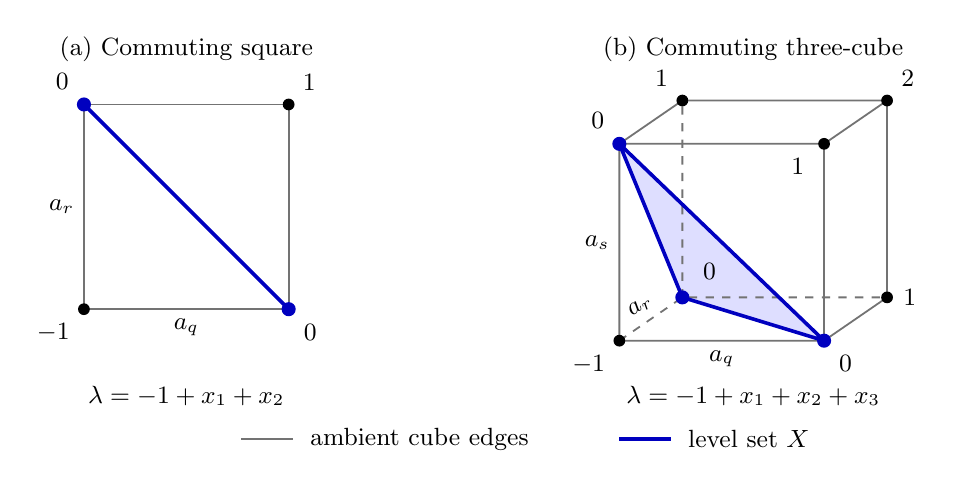
\begin{tikzpicture}[
  font=\small, line join=round,
  ambient/.style={draw=black!55,line width=.65pt},
  level/.style={draw=blue!75!black,line width=1.3pt},
  dot/.style={circle,fill=black,inner sep=1.5pt},
  zero/.style={circle,fill=blue!75!black,inner sep=1.8pt}]
  \begin{scope}[shift={(0,.4)}]
    \coordinate (A) at (0,0);
    \coordinate (B) at (2.6,0);
    \coordinate (C) at (0,2.6);
    \coordinate (D) at (2.6,2.6);
    \draw[ambient] (A)--(B)--(D)--(C)--cycle;
    \draw[level] (B)--(C);
    \node[dot,label=below left:$-1$] at (A) {};
    \node[zero,label=below right:$0$] at (B) {};
    \node[zero,label=above left:$0$] at (C) {};
    \node[dot,label=above right:$1$] at (D) {};
    \node[below] at (1.3,0) {$a_q$};
    \node[left] at (0,1.3) {$a_r$};
  \end{scope}
  \node at (1.3,3.7) {(a) Commuting square};
  \node at (1.3,-.7) {$\lambda=-1+x_1+x_2$};
  \begin{scope}[shift={(6.8,0)}]
    \coordinate (O) at (0,0);
    \coordinate (Q) at (2.6,0);
    \coordinate (R) at (.8,.55);
    \coordinate (S) at (0,2.5);
    \coordinate (QR) at (3.4,.55);
    \coordinate (QS) at (2.6,2.5);
    \coordinate (RS) at (.8,3.05);
    \coordinate (QRS) at (3.4,3.05);
    \fill[blue!13] (Q)--(R)--(S)--cycle;
    \draw[ambient,dashed] (O)--(R)--(QR) (R)--(RS);
    \draw[ambient] (O)--(Q)--(QR)--(QRS)--(RS)--(S)--cycle
      (Q)--(QS)--(S) (QS)--(QRS);
    \draw[level] (Q)--(R)--(S)--cycle;
    \node[dot,label=below left:$-1$] at (O) {};
    \node[zero,label=below right:$0$] at (Q) {};
    \node[zero,label={[xshift=2pt,yshift=1pt]above right:$0$}]
      at (R) {};
    \node[zero,label=above left:$0$] at (S) {};
    \node[dot,label=right:$1$] at (QR) {};
    \node[dot,label={[xshift=-2pt]below left:$1$}] at (QS) {};
    \node[dot,label=above left:$1$] at (RS) {};
    \node[dot,label=above right:$2$] at (QRS) {};
    \node[below] at (1.3,0) {$a_q$};
    \node[left] at (0,1.25) {$a_s$};
    \path (O)--node[above,sloped,pos=.48] {$a_r$} (R);
  \end{scope}
  \node at (8.5,3.7) {(b) Commuting three-cube};
  \node at (8.5,-.7) {$\lambda=-1+x_1+x_2+x_3$};
  \draw[ambient] (2,-1.25)--(2.65,-1.25);
  \node[right] at (2.75,-1.25) {ambient cube edges};
  \draw[level] (6.8,-1.25)--(7.45,-1.25);
  \node[right] at (7.55,-1.25) {level set $X$};
\end{tikzpicture}
\caption{Integer slices of cubes; vertex labels are heights. The blue
diagonal and triangle are an edge and a two-simplex of $X$. Each
generator increases height by one. Initial height $-2$ gives the other
triangular slice, at $x_1+x_2+x_3=2$.}
\label{fig:level-slices}
\end{figure}

The edge and triangular-word descriptions belong to the presentation
framework of Dicks and Leary \cite[Theorem~1 and Proposition~2]{DicksLeary1999}.
We now pass from the level geometry to the precise algebraic input for
Theorem~\ref{thm:presentation}. The finite cell orbits will give finite
alphabets, and acyclicity in both dimensions one and two will give an
isomorphism onto the cycle module, not merely a collection of generators.

\subsection{The group and its boundary basis}

\begin{proposition}\label{prop:model}
The finite flag complex $L$, its nontrivial representation
$\alpha:\pi_1(L)\to H$, and the group $G$ of
\eqref{eq:height-kernel} have the following properties.
\begin{enumerate}
\item $G$ is countable, finitely generated, and residually finite,
      with $\cdim(G)=2$ and $\gdim(G)\le3$.
\item $G$ acts freely on the integrally acyclic two-dimensional
      simplicial complex $X$ of \eqref{eq:zero-level}.  The action
      has finitely many cell orbits and one vertex orbit, identified
      with $G$ acting on itself on the left.
\item There is a finite generating alphabet $S$ for $G$ and a
      finite indexed list $\mathcal D$ of words trivial in $G$ such
      that, for $\Lambda=\Z[G]$, the graph of $X$ has edges
      $g\to gs$ and
      \begin{equation}\label{eq:model-resolution}
       0\longrightarrow\Lambda^{(\mathcal D)}
       \xrightarrow{\ \partial_2\ }\Lambda^{(S)}
       \xrightarrow{\ \partial_1\ }\Lambda
       \xrightarrow{\ \mathrm{aug}\ }\Z\longrightarrow0
      \end{equation}
      is exact, with $\partial_1(e_s)=s-1$ and
      $\partial_2(e_z)=[z]$.  Here $[z]$ is the oriented edge chain
      of the triangular boundary word $z$ based at $1$.
      In particular, the chains $[z]$, $z\in\mathcal D$, are a
      free $\Lambda$-basis of $\ker\partial_1$.
\end{enumerate}
\end{proposition}

\begin{proof}
The first two lemmas supply $L$, $\alpha$, and residual finiteness.
The cubical deck action restricts to $G$ on $X$.  It preserves the
cell structure just described, and no nonidentity element stabilizes
a cell: such an element would preserve its unique ambient open cube
in $E$, hence also that cube's initial vertex.  The action is free,
being the restriction of a deck action.  Vertices of $X$ are exactly
the elements of $G$, so there is one vertex orbit.

There are only finitely many cell orbits.  An ambient cube is
specified by its clique of directions and its initial vertex; a
nonempty integer slice has only finitely many possible relative
heights.  Two initial vertices of the same height differ by left
multiplication by an element of $G$.  Hence the finite list of
cliques and possible relative heights accounts for all the orbits.
The quotient $Y=X/G$ is thus a finite complex with one vertex, and
$X\to Y$ is a regular $G$-cover.  One can obtain this covering by
restricting $E\to E/G$.

Choose orientations for the edge orbits.  For each orbit choose its
oriented lift starting at $1$, and call its endpoint $s\in G$.
Keep different edge orbits as different letters even if their
values coincide; this defines $S$.  Left translation identifies
every oriented edge with $g\to gs$.  Connectedness of $X$ implies
that its graph is connected, so $S$ generates $G$.

For each triangle orbit choose an orientation, a starting corner,
and the lift having that corner at $1$.  Reading its boundary gives
a word $z$ on $S$, necessarily trivial in $G$.  These indexed words
form $\mathcal D$.  The cellular chains of $X$, with the chosen cell
orbit representatives, are precisely the free modules in
\eqref{eq:model-resolution}.  Acyclicity makes the augmented chain
complex exact.  In particular, $H_2(X;\Z)=0$ and the absence of
three-cells make $\partial_2$ injective, which gives the asserted
basis rather than only a spanning set.

This free resolution proves $\cdim(G)\le2$.  To obtain the
opposite inequality, choose a two-simplex of $L$ with vertices
$q,r,s$.  The three corresponding commuting generators form an
embedded $\Z^3$ in $P$: their map from $\Z^3$ is injective after
abelianization in $\Z^V$.  Its height kernel is a subgroup
$\Z^2\subset G$.  Cohomological dimension cannot increase upon
restriction to a subgroup, because a free group-ring module remains
free over the subgroup ring, and consequently projective modules
remain projective.  The torus resolution gives
$H^2(\Z^2;\Z)\cong\Z$, so $\cdim(G)\ge2$.

Finally, $P$ is finitely generated, hence countable, and so is $G$.
The contractible three-dimensional complex $E$ is also a free
$G$-complex; the quotient $E/G$ is a three-dimensional $K(G,1)$.
Thus $\gdim(G)\le3$, completing the proof.
\end{proof}
